%! Author = chouheiwa
%! Date = 2022/11/02

% Preamble
\documentclass[UTF8]{article} %article 文档
\usepackage{ctex}  %使用宏包(为了能够显示汉字)
\usepackage{hyperref}
\usepackage{graphicx}
\usepackage{geometry}
\geometry{a4paper,scale=0.8}
\usepackage{listings}
\usepackage{color}
\definecolor{dkgreen}{rgb}{0,0.6,0}
\definecolor{gray}{rgb}{0.5,0.5,0.5}
\definecolor{mauve}{rgb}{0.58,0,0.82}
\lstset{frame=tb,
    language=Python,
    aboveskip=3mm,
    belowskip=3mm,
    showstringspaces=false,
    columns=flexible,
    basicstyle={\small\ttfamily},
    numbers=left,%设置行号位置none不显示行号
%numberstyle=\tiny\courier, %设置行号大小
    numberstyle=\tiny\color{gray},
    keywordstyle=\color{blue},
    commentstyle=\color{dkgreen},
    stringstyle=\color{mauve},
    breaklines=true,
    breakatwhitespace=true,
    escapeinside=``,%逃逸字符(1左面的键),用于显示中文例如在代码中`中文...`
    tabsize=4,
    extendedchars=false %解决代码跨页时,章节标题,页眉等汉字不显示的问题
}

% Packages
\usepackage{amsmath}
\usepackage{amsthm}
\usepackage{amssymb}
\usepackage{mathtools}

% Document
\title{机器学习课程作业2-问题1}
\author{chouheiwa}
\date{2022/11/02}
\linespread{1.5}
\begin{document}
    \maketitle
    \tableofcontents


    \section{第一问}
    这里无法避免使用到矩阵的算法,以及绘图的算法,所以代码中会额外需要使用到numpy(用以进行数学运算)和matplotlib(用以生成和绘制相关散点图及分界线图)这两个库。

    已知三个正态分布函数$N_1(\mu_1, \Sigma_1)$, $N_2(\mu_2, \Sigma_2)$,$N_3(\mu_3, \Sigma_3)$,具体参数如下:

    \[
        \Sigma_1 = \Sigma_2 = \Sigma_3 = \left[
            \begin{matrix}
                1.2 & 0.4 \\
                0.4 & 1.8
            \end{matrix}
            \right]
    \]

    \[
        \mu_1 =  \left[
            \begin{matrix}
                0.1 \\
                0.1
            \end{matrix}
            \right]\text{ , }
        \mu_2 =  \left[
            \begin{matrix}
                2.1 \\
                1.9
            \end{matrix}
            \right]\text{ , }
        \mu_3 = \left[
            \begin{matrix}
                -1.5 \\
                2.0
            \end{matrix}
            \right]
    \]

    按照随机样本生成规则为:前两个样本使用 N2 生成,第三个样本使用 N1 生成,第四个样本使用 N3 生成。重复上述规则生成 500 个样本。
    随机样本遵循的概率密度函数建模为混合模型如下:
    \[
        p(x) = \sum_{i=1}^3 P_i N_i(\mu_i, \Sigma_i)
    \]

    我们可以使用如下两种方法生成样本集合:
    \begin{enumerate}
        \item 按照题目的生成规则进行生成,对应为\href{run:generate_data.py}{generate\_data.py}文件中的函数generate\_data,具体生成逻辑可以参考代码注释。
        \item 按照题目的生成规则对应进行数据分割,计算出种类分布规则数量,随后进行生成,对应为\href{run:generate_data.py}{generate\_data.py}文件中的函数generate\_data,具体生成逻辑可以参考代码注释。
    \end{enumerate}

    生成的数据集合如下图所示:

    \begin{minipage}[t]{0.5\linewidth}
        \centering
        \includegraphics[width=\linewidth]{../images/data}
    \end{minipage}


    \section{第二问}
    正态分布又被称为高斯分布。接下来均用高斯分布去替代正态分布。

    \subsection{高斯分布}
    多维高斯分布的概率密度函数为:
    \begin{equation}
        N(x;\mu, \Sigma) = \frac{1}{(2\pi)^{\frac{d}{2}}|\Sigma|^{\frac{1}{2}}}\exp\left(-\frac{1}{2}(x-\mu)^T\Sigma^{-1}(x-\mu)\right) \label{eq:gaussian}
    \end{equation}
    其中:
    \begin{enumerate}
        \item $x$ 是一个 $N \times d$ 的向量,代表着 $N$ 组 $d$ 维的样本,本题中 $N=500$,$d=2$。
        \item $\mu$ 是一个 $1 \times d$ 的向量,代表着对应维度的均值向量(数学期望)。
        \item $\Sigma$ 是一个 $d \times d$ 的矩阵,代表着模型的协方差矩阵。
    \end{enumerate}

    \subsection{Jensen不等式}
    Jensen不等式是一个非常重要的数学不等式,它的定义如下:
    \begin{equation}
        \mathbb{E}[f(x)] \geq f(\mathbb{E}[x]) \label{eq:jensen}
    \end{equation}

    \subsection{矩阵求导}
    多维高斯混合模型的求解需要借助矩阵和向量求导公式。如下部分是接下来推导过程中有可能使用到的公式:
    \begin{equation}
        \frac{\partial}{\partial x} (x-s)^T W (x-s) = -2W(x-s) \text{, (W 为对称矩阵)} \label{eq:matrix_derivation}
    \end{equation}

    \subsection{混合模型的概率密度函数}
    如题目中给定:
    \begin{align}
        p(x) &= \sum_{i=1}^3 P_i N_i(\mu_i, \Sigma_i) \notag \\
        &\text{将~\eqref{eq:gaussian}代入等式右边} \notag \\
        &= \sum_{i=1}^3 P_i \frac{1}{(2\pi)^{\frac{d}{2}}|\Sigma_i|^{\frac{1}{2}}}\exp\left(-\frac{1}{2}(x-\mu_i)^T\Sigma_i^{-1}(x-\mu_i)\right)  \label{eq:mixture_model}
    \end{align}
    这里$P_i$为第$i$个高斯分布模型的先验概率,显然有如下约束:
    \begin{equation}
        \sum_{i=1}^3 P_i = 1 \label{eq:sum_p}
    \end{equation}
    同时对于题目来说,我们需要去求解出每个高斯分布模型的参数 $P_i$、$\mu_i$、$\Sigma_i$,即参数也变成了未知数。这里将所有的参数都写成一个向量 $\theta$,则~\eqref{eq:mixture_model}可以写成如下形式:
    \begin{equation}
        p(x| \Theta) = \sum_{i=1}^3 P_i \frac{1}{(2\pi)^{\frac{d}{2}}|\Sigma_i|^{\frac{1}{2}}}\exp\left[-\frac{1}{2}(x-\mu_i)^T\Sigma_i^{-1}(x-\mu_i)\right] \label{eq:mixture_model_next}
    \end{equation}

    \subsection{EM算法}
    EM算法是一种迭代算法,其算法所解决的问题可简化为如下表述:
    \begin{enumerate}
        \item 获取一组包含 $N$(题目中为500,接下来的推导过程中不再重复提及了) 个样本的数据集合 $x$。
        \item 预先知晓(可以通过数据特点估计) $K$ (题目中给定数量为3,接下来的推导过程中不再重复提及了)个高斯分布混合模型用以进行数据拟合
        \item 目标任务为求解出每个高斯分布模型的参数 $\mu_i, \Sigma_i, P_i$。
    \end{enumerate}

    \subsubsection{似然估计}
    因为这里的每组数据均相互独立,所以用最大似然估计是最为直接的方法。而这里$N$个点数据的总概率为对应的每个数据点的概率乘积,即似然函数为:
    \begin{align}
        p(x|\Theta) &= \prod_{i=1}^N p(x_i| \Theta) \notag \\
        &= \prod_{i=1}^N \left[ \sum_{k=1}^K P_k N(x_i|\mu_k, \Sigma_k) \right]
    \end{align}

    使用对数形式对似然函数进行优化,可以把乘积变为求和:

    \begin{equation}
        L(x|\theta) = \sum_{i=1}^N \ln \left[ \sum_{k=1}^K P_k N_i(x_i|\mu_k, \Sigma_k) \right] \label{eq:likelihood_ln}
    \end{equation}

    这里使用最大似然估计的目的是为了求解出参数 $\Theta$,即将 $\Theta$ 作为自变量代入 ~\eqref{eq:likelihood_ln},并求解出似然函数的极大值,即可得到参数 $\Theta$ 的更优解,同时使用对数形式对于最大似然估计并无影响,因为对数函数是单调递增的,所以对数函数的最大值与原函数的最大值相同。
    \begin{equation}
        \Theta \coloneqq \arg\max_{\Theta} L(x|\theta) \label{eq:likelihood_max}
    \end{equation}

    \subsubsection{隐参数}
    对于 ~\eqref{eq:likelihood_ln},直接求极值并不可行。

    EM算法采用迭代逼近的方法,每次迭代都会得到一个更优的参数估计值,直到达到某个终止条件为止。帮助迭代过程,其提出了隐参数 $z$,每次迭代的时候,可以先使用上一次的参数计算隐参数 $z$ 的分布,然后再使用隐参数 $z$ 的分布计算参数的分布,这样就可以得到一个更优的参数估计值。

    对于高斯混合模型,隐参数 $z$ 的分布可以使用如下形式:$z \in 1,2,\dots,K$ 。其主要用于描述当计算出 当获得$K$组高斯模型的参数后,每个数据点属于哪个高斯模型的概率分布。即对于每个数据点 $x_i$,其属于第 $z$ 个高斯模型的概率为:
    $p(z|x_i,\mu_k,\Sigma_k)$
    该点对应的混合高斯模型的概率为:
    \begin{equation}
        p(x_i|\theta) = \sum_{k=1}^K p(z=k) p(x_i|z=k,\mu_k,\Sigma_k) \label{eq:z_gaussian_mixture}
    \end{equation}

    对比题目中给定分布概率$p(x_i|\theta) = \sum_{k=1}^K P_k N(x_i;\mu_k, \Sigma_k)$,可以看出 $P_k$即为$z$的先验分布$p(z=k)$:
    \begin{equation}
        P_k = p(z=k) \label{eq:z_prior}
    \end{equation}
    在$z=k$条件下,$x_i$的的条件概率也就是第k个高斯模型的概率密度函数:
    \begin{equation}
        p(x_i|z=k,\mu_k,\Sigma_k) = N(x_i;\mu_k, \Sigma_k) \label{eq:z_conditional}
    \end{equation}

    使用隐参数 $z$ 代入对数似然函数~\eqref{eq:likelihood_ln}。同时加入冗余项:$p(z=k|x_i,\mu_k,\Sigma_k)$($z$ 在数据 $x_i$ 和 高斯分布$k$下的后验概率),可得:
    \begin{align}
        L(x|\theta) &= \sum_{i=1}^N \ln \left[ \sum_{k=1}^K p(z=k) p(x_i|z=k,\mu_k, \Sigma_k) \right] \notag \\
        &= \sum_{i=1}^N \ln \left[ \sum_{k=1}^K p(z=k|x_i,\mu_k,\Sigma_k) \frac{p(z=k) p(x_i|z=k,\mu_k, \Sigma_k)}{p(z=k|x_i,\mu_k,\Sigma_k)} \right] \label{al:likelihood_ln_z}
    \end{align}

    \subsubsection{简化对数似然函数}
    \begin{align}
        \text{令} u &= \frac{p(z=k) p(x_i|z=k,\mu_k, \Sigma_k)}{p(z=k|x_i,\mu_k,\Sigma_k)} \notag \\
        \text{令} f(u) &= \ln u \notag \\
        \text{令} E(u) &= \sum_{k=1}^K p(z=k|x_i,\mu_k,\Sigma_k)u \notag \\
        \text{则} L(x|\theta) &= \sum_{i=1}^N f\left[ E(u) \right] \notag \\
        \text{结合 ~\eqref{eq:jensen} 有} L(x|\theta) &\geq E\left[ f(u) \right] \notag \\
        &= \sum_{i=1}^N \sum_{k=1}^K p(z=k|x_i,\mu_k,\Sigma_k) \ln \frac{p(z=k) p(x_i|z=k,\mu_k, \Sigma_k)}{p(z=k|x_i,\mu_k,\Sigma_k)} \label{al:likelihood_ln_z_simplify}
    \end{align}
    其中,等式右侧提供给了对数似然函数一个下界。接下来使用贝叶斯准则,可以推导出后验概率$p(z=k|x_i,\mu_k,\Sigma_k)$:

    \begin{align}
        p(z=k|x_i,\mu_k,\Sigma_k) &= \frac{p(z=k) p(x_i|z=k,\mu_k, \Sigma_k)}{\sum_{k=1}^K p(z=k) p(x_i|z=k,\mu_k, \Sigma_k)} \notag \\
        &= \frac{P_k N(x_i;\mu_k, \Sigma_k)}{\sum_{k=1}^K P_k N(x_i;\mu_k, \Sigma_k)} \notag \\
        \text{令} \omega_{i,k} &= p(z=k|x_i,\mu_k,\Sigma_k) \notag \\
        &= \frac{P_k N(x_i;\mu_k, \Sigma_k)}{\sum_{k=1}^K P_k N(x_i;\mu_k, \Sigma_k)} \label{eq:omega}
    \end{align}

    此时可代入~\eqref{eq:omega}对数似然函数~\eqref{al:likelihood_ln_z_simplify}中得:
    \begin{equation}
        L(x|\theta) \geq \sum_{i=1}^N \sum_{k=1}^K \omega_{i,k} \ln \frac{p(z=k) p(x_i|z=k,\mu_k, \Sigma_k)}{\omega_{i,k}} \label{eq:likelihood_ln_z_simplify_omega}
    \end{equation}

    于是我们可以使用EM算法不断优化下界,从而逼近似然函数。优化目标函数为:
    \begin{equation}
        \mathcal{Q}(\theta, \theta^t) = \sum_{i=1}^N \sum_{k=1}^K \omega_{i,k} \ln \frac{p(z=k) p(x_i|z=k,\mu_k, \Sigma_k)}{\omega_{i,k}} \label{eq:likelihood_ln_z_simplify_target_function}
    \end{equation}

    其中,函数式表明: 在第 $t$ 次迭代中,获得参数 $\theta^t$ 时,可以计算出隐参数的后验概率$\omega_{i,k}^t$,将隐参数代回$\mathcal{Q}(\theta, \theta^t)$中,进行最大似然优化,便可得到更优的参数 $\theta^{t+1}$。

    \subsubsection{EM算法步骤: E-Step}
    将~\eqref{eq:likelihood_ln_z_simplify_target_function}展开,得到:
    \begin{equation}
        \mathcal{Q}(\theta, \theta^t) = \sum_{i=1}^N \sum_{k=1}^K \omega_{i,k} \ln \frac{P_k}{\omega_{i,k} \sqrt{(2\pi)^d + |\Sigma|}} \exp \left[ - \frac{1}{2} (x_i - \mu_k)^T \Sigma_k^{-1} (x_i - \mu_k) \right] \label{eq:likelihood_ln_z_simplify_target_function_expand}
    \end{equation}

    其中:
    \begin{enumerate}
        \item $x_i$: $1 \times d$维向量
        \item $P_k$: $P_k \in (0, 1)$
        \item $\mu_k$: $1 \times d$维向量
        \item $\Sigma_k$: $d \times d$维矩阵
        \item $\omega_{i,k}^t$: $N \times K$维矩阵
    \end{enumerate}
    这里更新目标函数 ~\eqref{eq:likelihood_ln_z_simplify_target_function}:
    \begin{equation}
        \mathcal{Q}(\theta, \theta^t) = \sum_{i=1}^N \sum_{k=1}^K \omega_{i,k}^t \left[ \ln P_k^t - \ln \omega_{i,k}^t - \frac{d}{2} \ln 2\pi - \frac{1}{2} ln |\Sigma_k| - \frac{1}{2} (x_i - \mu_k)^T \Sigma_k^{-1} (x_i - \mu_k) \right] \label{eq:likelihood_ln_z_simplify_target_function_t}
    \end{equation}

    \subsubsection{EM算法步骤: M-Step}

    \paragraph{更新$P_k$:} ~\\
    \begin{equation}
        P_k^{t+1} = \frac{\sum_{i=1}^N \omega_{i,k}^t}{N}\label{eq:P_k^{t+1}}
    \end{equation}

    \paragraph{更新$\mu_k$:} ~\\
    \begin{equation}
        \mu_k^{t+1} = \frac{\sum_{i=1}^N \omega_{i,k}^t x_i}{\sum_{i=1}^N \omega_{i,k}^t}\label{eq:mu_k^{t+1}}
    \end{equation}

    \paragraph{更新$\Sigma_k$:} ~\\
    \begin{equation}
        \Sigma_k^{t+1} = \frac{\sum_{i=1}^N \omega_{i,k}^t (x_i - \mu_k^{t+1})^T (x_i - \mu_k^{t+1})}{\sum_{i=1}^N \omega_{i,k}^t}\label{eq:Sigma_k^{t+1}}
    \end{equation}

    \subsubsection{EM算法步骤流程}

    算法步骤流程图如下:

    \begin{minipage}[t]{0.5\linewidth}
        \centering
        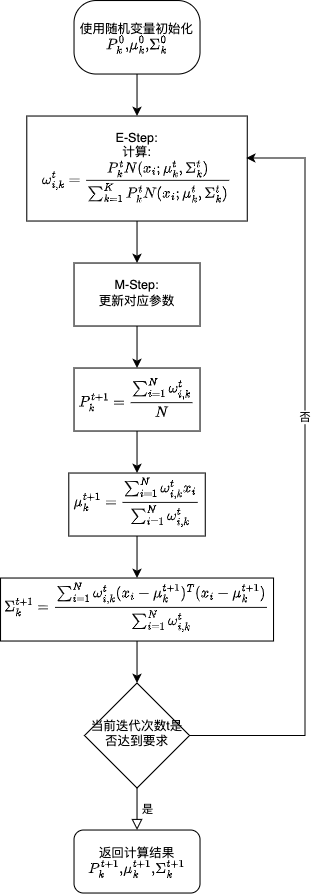
\includegraphics[width=\linewidth]{GMM-EM算法更新流程图.drawio}
    \end{minipage}

    真正算法实现在\href{run:gmm_em.py}{gmm\_em.py}文件中的函数gmm\_em,具体生成逻辑可以参考代码注释。

    \subsubsection{其他}
    由于EM算法求解出的是K个高斯分布,其很可能与题目中的给定顺序分布并不一致,因此需要额外的步骤将其转换为题目中的顺序分布。这里使用均值期望$\mu$做为判别依据,将计算出的K个高斯分布的$\hat{\mu}$与题目中的顺序分布$\mu$进行比较,将$\hat{\mu}$与$\mu$最接近的高斯分布的参数作为题目中的顺序分布的参数。

    算法实现在\href{run:main.py}{main.py}文件中的函数calculate\_order,具体生成逻辑可以参考代码注释。

    \subsubsection{实验结果}
    这里使用的初始值为:
    \input{result.tex}

    其中,$\hat{\mu}$的值随随迭代次数变化曲线如下图所示:

    \includegraphics[width=\linewidth]{../images/mu_iteration}

    可以看出,$\hat{\mu}$的值在约800次迭代后基本稳定,这里设置1000次迭代是一定量的冗余从而可以更好的保证结果的稳定性。

    这里不在画出其他参数值与迭代次数的变化曲线了

    \section{第三问}
    通过多次运行随机不同的初始值$\hat{\mu}^{(0)})$,可以得到若干个不同的结果,误差也各不相同。

    结合第二问中求解过程,可知,对于EM算法,核心思想是通过迭代的方式,不断地更新参数,使得目标函数的值不断地减小,更新参数的过程,是求令其偏导数等于0去求解的,而偏导数等于0的解,其实是一个局部最优解,而不是全局最优解,因此,EM算法的结果,是一个局部最优解,而不是全局最优解。因此我们重复尝试不同的初始$\hat{\mu}^{(0)})$,可以使$\theta$落入不同的局部最优解中。

    题目中由于知晓其正态分布的均值,因此我们的优化其实是可以将$\hat{\mu}^{(0)})$越来越趋近真实值$\mu$的,因此,我们可以通过多次尝试,使得$\hat{\mu}$越来越接近$\mu$,从而使得误差越来越小。

    若真实情况下,我们无法知晓其具体正态分布函数的参数值的,因此对于这类问题的误差。我们还需要在计算出正态分布函数的参数值后,还应带回$X$的数据集并给出对应分类,做多次尝试,并取使分类错误点最低的分布分类参数。


\end{document}